%!TEX root = ../TAMUTemplate.tex
%%%%%%%%%%%%%%%%%%%%%%%%%%%%%%%%%%%%%%%%%%%%%%%%%%%
%
%  New template code for TAMU Theses and Dissertations starting Fall 2016.
%
%  Author: Sean Zachary Roberson
%	 Version 3.16.09
%  Last updated 9/12/2016
%
%%%%%%%%%%%%%%%%%%%%%%%%%%%%%%%%%%%%%%%%%%%%%%%%%%%

%%%%%%%%%%%%%%%%%%%%%%%%%%%%%%%%%%%%%%%%%%%%%%%%%%%%%%%%%%%%%%%%%%%%%%%
%%%                           SECTION III
%%%%%%%%%%%%%%%%%%%%%%%%%%%%%%%%%%%%%%%%%%%%%%%%%%%%%%%%%%%%%%%%%%%%%%


\chapter{\uppercase {Particle-Flow Objects}}

Particle detectors like CMS are, in essence, like large cameras; taking high resolution pictures of the paths of the decay products coming from proton-proton collisions.
Each collision will produce various types of SM, and maybe beyond the Standard Model (BSM), particles which will have unique behaviors as they traverse the detector.
Fig.~\ref{fig:particle_flow} shows how various types of particles interact with the CMS detector and its different sub-detector materials.
All of the charged particles (\ie electrons, muons, and charged hadrons) will deposit some energy in the tracker, while neutral particles (\ie photons and neutral hadrons) will not.
Electrons and photons will deposit all of their energy inside of the ECAL while hadrons, both charged and neutral, will deposit most of their energy in the HCAL.
Muons are the only visible particle which will be able to travel to the muon chambers.
Neutrinos will pass through all layers of the detector unseen and their presence must be inferred by missing transverse energy (\MET or \ETslash); the idea being that if the sum of the transverse momentum is not conserved, then that missing momentum must correspond to at least one unseen particle.

Even after acquiring the sparsely filled images of energy deposits, sophisticated reconstruction algorithms must turn these into an image of particles and higher level physics objects (i.e. jets, taus, MET).
The subsystems (i.e. one section and technology of the muon system) of each sub-detector create reconstructed hits (RecHits) containing the local information of the energy deposits.
From there the subsystem information is combined to form local physics objects (i.e. track segments in the muon sub-detector).
The next step is a type of global event description (GED), wherein particles are created and classified based on the linking of the various sub-detector objects.
The particles can be classified as electrons, photons, muons, charged hadrons, or neutral hadrons.
This so-called particle-flow (PF) algorithm is on of the hallmarks of the CMS experiment~\cite{CMS-PRF-14-001} and is capable of yielding much better measurements than traditional, single sub-detector algorithms.
This analysis will make use of electrons, muon, jets, and \ETslash.
Much more can be written about the reconstruction of each of these object, but this is probably beyond the scope of this propose.
Instead each of these objects and their reconstruction will be discussed in detail in the thesis.

\begin{figure}[!hbt]
	\centering
	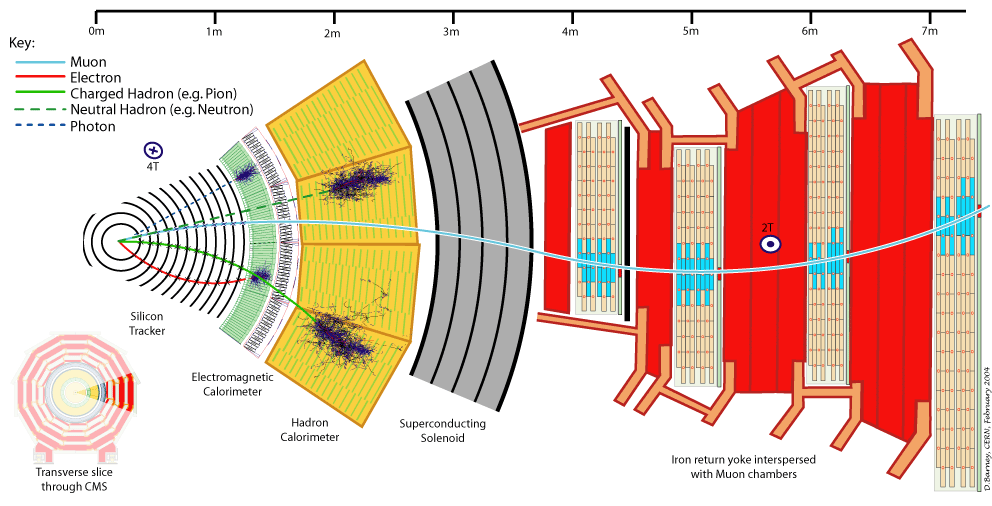
\includegraphics[width=0.95\textwidth]{\figpath/Chapter3/ParticleFlow}
	\caption{Cross-sectional view of the CMS detector with all of the sub-detectors labeled. The different colored lines represent how various types of particles interact with the sub-detectors and may or may not be bent by the magnetic field~\cite{CMSSlice}.}
	\label{fig:particle_flow}
\end{figure}

